\chapter{Results and Evaluation}

\section{EDB Analysis}\label{edb analysis}
A substantial part of my work was the exploiting of available sources which includes the EDB and scraped epidemiological news. In the following I introduce how I managed to recover most of the information in the EDB for my further analyzes and how I managed to scrape a large amount epidemiological data with a limited time profile.

\subsection{Source Determination}
Before I could train a classifier to detect relevant articles or extract meaningful key words from texts, I needed to create a labeled dataset from the EDB. The entries in the EDB were the positive labels, but I lacked the negative examples, i.e., the articles that were read by the epidemiologists but were not considered. However, writing a scraper can be time consuming so I needed to narrow down the, at that moment, 75 sources of the EDB.

For this, I extracted all URLs from the EDB and clustered them to identify sources that were used more often than others  (Fig . \ref{fig:netloc}). Then, I focused only on the most used sources that were also unproblematic to scrape (Fig. \ref{table:INIGsources}). I determined the importance of the articles by binning the referenced Netlocs from the EDB and chose the highest ranking ones. The difficulty, on the other hand, I found by exemplary text extractions. With this information at hand I knew which sources to scrape. The EDB contained the work of INIG throughout the year 2018. Thus, I needed to extract all articles of the year 2018 from the determined sources that are partly shown in Tab. \ref{table:INIGsources}.

\begin{figure}[h!]
    \centering
    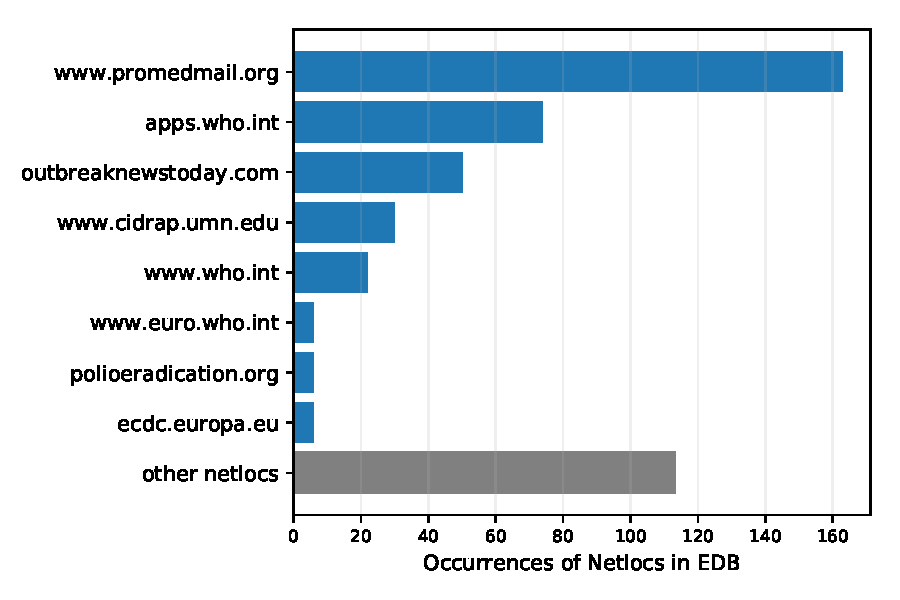
\includegraphics[scale=0.5]{netloc.pdf}
    \caption{KJhaskdj.}
    \label{fig:netloc}
\end{figure}


\begin{table}[h!]
  \centering
  \begin{tabular}{@{}cccc@{}}
    \toprule
    \textbf{Source} & \textbf{Data Format} & \textbf{Data Quality} & \textbf{Accesibility}\\
    \midrule
    \href{http://www.cidrap.umn.edu/}{CIDRAP} & HTML & Mixed content & Intermediate \\
    \href{http://www.promedmail.org/}{ProMED Mail} & HTML & Only relevant & Easy\\
    \href{http://www.who.int/csr/don/en/}{WHO DONs} & HTML & Only relevant & Easy \\
    EIOS daily digest & Email & Only relevant & Hard \\
    \href{http://outbreaknewstoday.com/}{OutbreakNewsToday} & HTML & Mixed content & Intermediate\\
    ECDC Report & Email & Only relevant & Hard \\
    \href{http://www.afro.who.int/fr/health-topics/disease-outbreaks/outbreaks-and-other-emergencies-updates}{WHO Afro Bulletin} & PDF & Only relevant & Hard \\
    \href{http://www.eurosurveillance.org/content/eurosurveillance/browse}{EuroSurveillance} & PDF and HTML & Mixed content & Intermediate \\
    \href{http://www.who.int/wer/en/}{WHO WER} & PDF & Mixed content & Hard\\
    \href{https://ecdc.europa.eu/en/threats-and-outbreaks/reports-and-data/weekly-threats}{ECDC CDTR} & PDF & Only relevant & Intermediate \\
    \href{http://www.emro.who.int/pandemic-epidemic-diseases/information-resources/weekly-epidemiological-monitor.html}{WHO EMRO} & PDF & Mixed content & Hard \\
    \href{https://www.paho.org/hq/index.php?option=com_content&view=article&id=14044:epidemiological-alerts-archive-by-year-2018&Itemid=72203&lang=en}{WHP PAHO} & PDF & Only relevant & Intermediate\\
    \bottomrule
  \end{tabular}
  \caption{A list of the obligated sources for the daily screening of INIG and the data type of the source. Furthermore, I assessed the sources for their quality, i.e., whether they only contain information relevant for epidemiological surveillance or also research findings and ongoing projects (mixed content). After exemplary testing, I rated the difficulty to extract analyzable text from these sources where \textsl{easy} posed no difficulty, \textsl{intermediate} would have required additional work but is promising to function and \textsl{hard} was unsure whether it could work satisfactorily.}
  % \setlength{\tabcolsep}{1.5em}
\label{table:INIGsources}
\end{table}

\subsection{Data Quality}
Due to the unrestrained column settings, every entry in the EDB was free text with spelling mistakes and different formatting. The transferral of the EDB into a controlled vocabulary was a vital steps since it made more data points usabel. Tab. \ref{table:preprocessing performance} shows that the preprocessing made up to 100 EDB entries accessible per keyword.

\begin{table}
  \centering
  \caption{Performance evaluation of the EDB preprocessing per key word. The table shows the amount of valid and invalid entries before and after preprocessing was applied. The EDB in sum has 557 entries.  }
  \begin{tabular}{@{}cccc@{}}
    \toprule
    \textbf{Key Word} & \textbf{Valid Before} & \textbf{Valid After} & \textbf{Invalid After} \\
    & \textbf{Preprocessing} & \textbf{Preprocessing} & \textbf{Preprocessing} \\
    \midrule
    Date & 168 & 168 &  19 \\
    Case count & 299 & 394 &  18 \\
    Country & 355 & 494 &  17 \\
    Disease & 231 & 332 & 16 \\
    \bottomrule
  \end{tabular}
  \label{table:preprocessing performance}
\end{table}

\section{Key Information Extraction}
\section{Article Recommendation}
